\section{Implementation}
\label{sect:kegg_implementation}

The implementations for \mawapp and \keggapp similar in many ways, but they have
some important differences. Development on \keggapp was begun a year after
\mawapp and provided opportunities to improve on the interface, design, and
implementation of the pathway viewing app concept.

The improved design was made possible partially by new features introduced into
the iPad development stack in 2011 with the release of iOS 5. The most important
change was ``automatic reference counting,'' which moves memory management
responsibility from the programmer to the compiler. 

\keggappp architecture consists of a few well-defined components:

\begin{itemize}

    \item Top-level user interface such as the master-detail view
    
    \item Web service request classes that make HTTP requests to the PathCase
        KEGG server, process the response, and notify other objects of the
        results

    \item Views of specific kinds of data such as pathways (the main graph
        view), pathway lists, organism hierarchies, web pages, and pathway nodes

    \item Encapsulated components for specific functionality such as reading the
        ENZYME database and generating dynamic layouts with graphviz

\end{itemize}

\subsection{Top-Level User Interface}
\label{sect:kegg_impl_top_level_ui}

To be written.

\subsubsection{Web Services: Server Side}

\subsection{Web Services}
\label{sect:kegg_impl_web_services}

There are four differences between the strategies of \mawapp and \keggapp
with respect to how web services are integrated into the application
architecture.

The first difference is that \keggapp does not download the entire PathCase
KEGG database at once. HTTP requests are made as new data is needed, and the
result is cached in the device's internal storage.

The second is in class hierarchy. \mawapp has methods in various data model
classes which are responsible for making an HTTP request and taking some action
based on its success or failure. \keggapp has a separate class for each web
service, named \texttt{PC<WebService>Fetcher}.

The third is how dependencies between requests are managed. \mawapp uses
mutexes to force the data update thread to wait before starting a request that
depends on a previous request. \keggappp web service classes fire events to
a central notification system when they have completed, and controller objects
check to see if any new web services should be invoked due to dependencies being
made available.

The fourth is in what sorts of transformations are done to the results of the
HTTP request. Unlike \mawapp, after the XML response has been parsed into
one or more KEGG internal objects, these objects are not serialized. In other
words, all objects generated by web services are built from the XML each time
they are needed. The XML response of the web service is the canonical
representation of the object.

These differences are summarized in figure
\ref{fig:kegg_impl_web_service_differences}.

\begin{figure}[hbt]
    \center{
        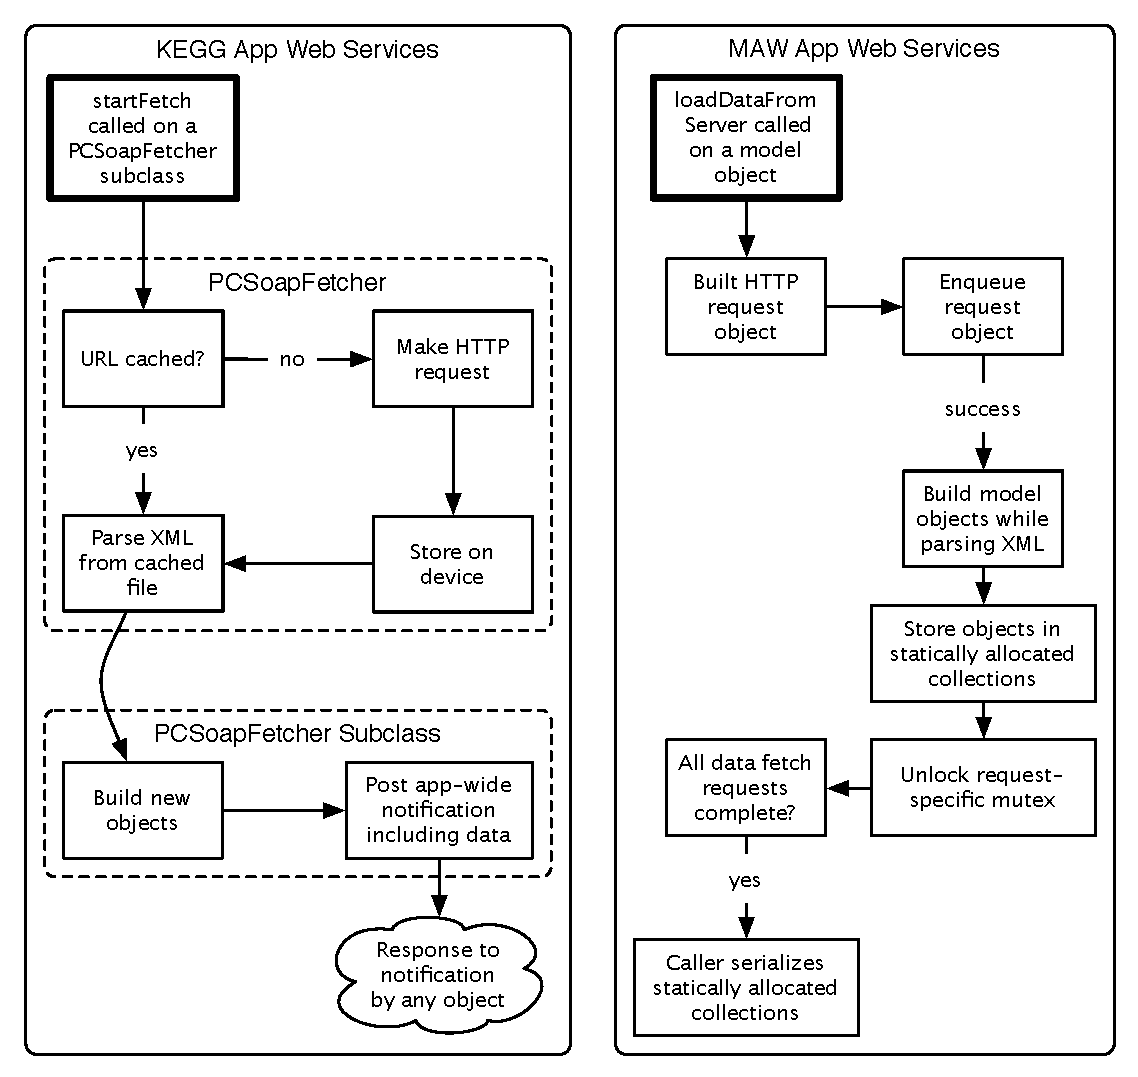
\includegraphics[width=\textwidth]{kegg/figures/web_services.pdf}}
    \caption{\label{fig:kegg_impl_web_service_differences} Side-by-side
    comparison of the typical life cycle of a \keggapp service request and a
    \mawapp web service request.}
\end{figure}

This model of web services would not necessarily work better for \mawapp,
which needs quicker access to much more interdependent data. When the data model
is serialized, it is simple to load it and traverse complex relationships. The
data handled by \keggapp, on the other hand, is not very interdependent, so
it is simpler to make the web service requests on demand and turn the XML into
objects in memory on the fly.

\subsection{Data Views}
\label{sect:kegg_impl_data_views}

These are also mostly boring to talk about. Each data view has a model (an
object which is being displayed such as a node, a pathway, or a list of
organisms), a view (a table, row of colored labels, a graph view, etc.), and a
controller (translating the model to the view and responding to UI and web
service events).

\subsubsection{Pathway Graph View}
\label{sect:kegg_impl_graph_view}

This will be an explanation of the \keggapp graph view and how it differs from
the \mawapp graph view. In short, it is more encapsulated and less dependent on
the rest of the data model.

\subsection{Reading the ENZYME Database}
\label{sect:kegg_impl_enzyme}

The ENZYME database is provided in a flat file format \cite{enzyme:enzuser}. This
format is not acceptable for random access behavior. To get around this issue, a
Python script translates the entire file into a SQLite database that is bundled
with \keggapp and queried by its code. (SQLite is a minimal implementation
of SQL intended to be used as a storage medium for single-instance applications
\cite{sqlite:main}.)

Access to the SQLite database is encapsulated in the \texttt{EKEnzyme} class. It
can be used by calling \texttt{[EKEnzyme enzymeForID:(NSString *)ECNumber]},
which returns an \texttt{EKEnzyme} object that has an instance variable for each
type of data in the ENZYME database entry.

\subsection{Dynamic Layouts with graphviz}
\label{sect:kegg_impl_graphviz}

PathCase KEGG contains human-curated frozen layouts for some pathways, but not
all. In order to display the pathways without frozen layouts, \keggapp
uses the graphviz library.

(Blurb about the graphviz project, what it does, etc.)

The layout functionality of graphviz is encapsulated in the \texttt{GVGraph}
class. An instance of this class represents a single graph. Nodes and edges are
added by calling methods on this class, which create \texttt{GVGraphNode} and
\texttt{GVGraphEdge} objects that contain only the information that is important
for generating a layout. They are completely separate from the graph view node
and edge objects that have additional information about color and edge arrow
shapes.

The call to graphviz is made when the \texttt{computeLayoutWithEngine:} method
is called on the \texttt{GVGraph} instance. (The single argument is a constant
representing the spring-based or hierarchical layout engine.) This method call
turns the \texttt{GVGraph}'s node and edge objects into graphviz objects, asks
graphviz to generate a layout, and reads the node positions from graphviz back
into the \texttt{GVGraphNode} and \texttt{GraphEdge} objects.

At this point, it is the caller's responsibility to read the position data from
\texttt{GVGraphNode} and \texttt{GraphEdge} into whatever objects it likes. In
the case of \keggapp, this is the graph view node and edge objects.
